\documentclass[12pt]{article}

\usepackage[margin=1in]{geometry}
\usepackage{amsmath,amssymb,latexsym,amsthm}
\usepackage{graphicx}
\usepackage{epstopdf}
\usepackage{hyperref}
\usepackage{xcolor}
\usepackage{verbatim}
\usepackage{subfigure}
\usepackage{caption}
\usepackage{multirow}
\usepackage{float}
\usepackage{setspace}
\usepackage{natbib}

\theoremstyle{definition}
\newtheorem{definition}{Definition}
\newtheorem{proposition}{Proposition}
\newtheorem{remark}{Remark}
\onehalfspacing

\title{Risk Aversion or Mistaken Beliefs?\\[6pt]
\large Three Martingales and More\thanks{This paper is the basis for
the inaugural David Backus Memorial Lecture.
Dave was a pioneer in the study of affine term structure models and
international risk sharing.
His 2001 paper with Foresi and Telmer on affine models of currency
pricing is a direct intellectual ancestor of the framework presented
here.
Dave was skilled at connecting theory to data in sophisticated ways. He was also extraordinarily generous as a colleague,
critic, and teacher.
I thank Jonathan Payne, Jiao Shi, and B\'alint Sz\H{o}ke for helpful discussions preceding my delivery of the Backus lecture,
and Ziyue Yang for criticisms of earlier drafts of this paper.}}

\author{Thomas J.\ Sargent\\[4pt]
\small New York University}

\date{March 2026}

\begin{document}

\maketitle

\begin{abstract}
This paper explores the confounding of risk aversion and mistaken beliefs
in asset pricing.  A likelihood ratio---a multiplicative martingale
increment---serves as the key mathematical object that connects
risk-neutral pricing, subjective belief distortions, and concerns about
model misspecification.  I describe three uses of likelihood ratios:
(i)~to encode a representative investor's risk aversion, following
Lucas and Hansen; (ii)~to represent mistaken beliefs of professional
forecasters, following Piazzesi, Salomao, and Schneider; and (iii)~to
capture fears of model misspecification, following Hansen and
Sz\H{o}ke.  I show how the third use, with a tilted discounted entropy
ball that accommodates concerns about particular parametric models
featuring long-run risk, can generate the state-dependent uncertainty
prices needed to explain hitherto puzzling term-structure movements.
\end{abstract}

\newpage
%\tableofcontents
%\newpage

%% ====================================================================
\section{Introduction}
\label{sec:intro}
%% ====================================================================



Long-standing puzzles about the term structure of interest rates that motivated some of Dave Backus's work motivate this paper too. I define a ``puzzle'' as a feature of the joint distribution of macroeconomic variables and asset returns implied by a ``standard'' benchmark macroeconomic model that is contradicted by U.S.\ time series data. In fact, the nominal yield curve usually slopes upward. The long-minus-short yield spread narrows before recessions and widens after them. Remarkably, long-term bond yields are nearly as volatile as short-term yields even though, under a rational expectations version of the expectations theory of the term structure, they should be much smoother averages of expected future short rates.\footnote{For influential research about the expectations theory of the term structure of interest rates before rational expectations was imposed, see Bierwag and Grove~(1967) and Meiselman~(1961).} This is Robert Shiller's (1979) ``volatility puzzle.''

Sargent~(1972, 1979) and Hansen and Sargent~(1991) tested cross-equation restrictions on vector autoregressions implied by the rational expectations theory of the term structure. They found some support for the theory's implications for conditional means, but also early hints of the difficulties with conditional second moments that Shiller emphasized. To resolve the volatility puzzle, risk prices---or something observationally equivalent---must be large, volatile, and state-dependent. What generates those state-dependent risk prices? Risk aversion? Wrong beliefs? Fears of model misspecification? Disentangling these possible sources is the topic of this paper.

Consequences of investors' \emph{risk aversion} and \emph{wrong beliefs} are
confounded in asset pricing data.  In a rational expectations model with a
risk-averse representative investor, higher mean returns compensate for
higher risks.  But if the rational expectations assumption is wrong because the representative investor holds wrong beliefs,
observed average returns depend on \emph{both} risk aversion \emph{and}
misunderstood return distributions.  Thus, wrong beliefs can contribute what, from the point of view of an econometrician's approximating model,
look like ``stochastic discount factor shocks.'' Does the presence of such ``shocks'' have the potential to explain observed countercyclical risk prices?


This paper organizes ideas around a single mathematical device: the
\emph{likelihood ratio}, a non-negative random variable with unit mean
that twists one probability distribution into another.
Much of the analysis draws on two papers:
Hansen, Sz\H{o}ke, Han, and Sargent~(2020), who construct
twisted probability models from tilted discounted entropy balls to
price model uncertainty, and Sz\H{o}ke~(2022), who estimates a
robust control model with cross-equation restrictions implied by a
representative agent's worst-case beliefs and evaluates its
implications for the yield curve and survey expectations.
Likelihood
ratios---equivalently, multiplicative martingale increments---appear in
at least four distinct roles in modern asset pricing:

\begin{table}[H]
\begin{center}
\begin{tabular}{lll}
\textbf{Probability}  & \textbf{Likelihood ratio} & \textbf{Describes} \\
\hline\\[-6pt]
Econometric  &  1 &  macro risk factors \\[4pt]
Risk neutral  & $m_{t+1}^\lambda $ & prices of risks  \\[4pt]
Mistaken &  $m_{t+1}^w $  & experts' forecasts  \\[4pt]
Doubtful & $m_{t+1} \in {\mathcal M} $ & misspecification fears  \\[4pt]
\end{tabular}
\end{center}
\caption{Four probability measures and associated likelihood ratios.
Each likelihood ratio takes the log-normal form
$m_{t+1}^b = \exp\bigl(-b_t' \varepsilon_{t+1} - \tfrac{1}{2} b_t' b_t \bigr)$
with $b_t = 0$, $\lambda_t$, $w_t$, or a worst-case distortion.}
\label{tab:four-measures}
\end{table}

The ``three martingales'' of my subtitle are cumulative likelihood
ratio processes $\{M_t\}$ formed from (i)~risk prices $\lambda_t$,
(ii)~belief distortions $w_t^*$, and (iii)~worst-case model distortions
$\tilde w_t$.  The ``and more'' refers to $\bar w_t$, the parametric
long-run risk worry that tilts the entropy ball.

The rest of this paper proceeds as follows.  Section~\ref{sec:risks-and-beliefs}
sets up a Gaussian statistical framework in which a likelihood ratio twists
probabilities while preserving a tractable structure.
Section~\ref{sec:asset-pricing} reviews rational-expectations asset
pricing and shows how a single likelihood ratio turns risk-neutral
pricing formulas into modern asset pricing formulas.
Section~\ref{sec:identification} discusses a parameter identification issue:
the same likelihood ratio can be interpreted as risk aversion or as
belief distortion. Section~\ref{sec:PSS} describes an approach of
Piazzesi, Salomao, and Schneider~(2015), who use survey data on
professional forecasters to decompose the likelihood ratio into a
smaller risk price and a belief distortion.
Section~\ref{sec:RE-limits} pauses to examine why rational expectations
may not be a good approximation when persistent dynamics make convergence
of learning slow.
Section~\ref{sec:robust} develops a robust control theory approach,
beginning with Hansen's formulation with a discounted entropy ball. Section~\ref{sec:tilted}
discusses Hansen and Sz\H{o}ke's tilted entropy ball that
accommodates concerns about parametric alternatives with more long-run
risk.  Section~\ref{sec:empirics} summarizes empirical results. Section~\ref{sec:motivation} describes how models 
of robustness impose powerful cross-equation restrictions that resemble those imposed by rational expectations models.
Section~\ref{sec:conclusion} concludes with reflections on why different interpretations and fits of these
joint probability distributions matter for macroeconomics. Appendix~\ref{sec:multiplier} describes some details
about multiplier preferences. 


%% ====================================================================
\section{Risks and Beliefs}
\label{sec:risks-and-beliefs}
%% ====================================================================

This section introduces the paper's central mathematical device: a
likelihood ratio that twists one probability distribution into another.
In a Gaussian setting, this twist amounts to shifting the mean of the
shock distribution by a vector~$\lambda$ while leaving the covariance
structure unchanged.  The resulting framework is deliberately
simple---it sets up the vocabulary and notation that will recur
throughout the paper.

Let $\varepsilon$ denote a vector of risks to be taken and priced.
Suppose that, under the econometrician's probability model,
$\varepsilon$ has a standard multivariate normal density:
\[
   \phi(\varepsilon)  \propto \exp\!\left(- \tfrac{1}{2}\,
       \varepsilon' \varepsilon\right), \qquad
       \varepsilon \sim {\mathcal N}(0,I).
\]
Define a \emph{likelihood ratio}
\[
   m(\varepsilon)  = \exp \!\left( -\lambda' \varepsilon
       - \tfrac{1}{2}\, \lambda' \lambda \right) \geq 0,
\]
which satisfies $E\, m(\varepsilon) = 1$ by construction.  The
\emph{twisted density}
\[
   \hat \phi(\varepsilon)  =  m(\varepsilon)\, \phi(\varepsilon)
   \propto \exp\!\left( - \tfrac{1}{2}\,
       (\varepsilon + \lambda)'(\varepsilon + \lambda)\right)
\]
is a ${\mathcal N}(-\lambda, I)$ density.  The \emph{relative entropy}
of the twisted density with respect to the baseline density is
\[
   E\bigl[ m(\varepsilon) \log m(\varepsilon) \bigr]
       = \tfrac{1}{2}\, \lambda'\lambda,
\]
a convenient measure of the statistical distance between the two models.

The vector $\lambda$ is the key object.  Depending on context it
represents risk prices, belief distortions, or worst-case mean
perturbations under model uncertainty.


%% ====================================================================
\section{Asset Pricing with Likelihood Ratios}
\label{sec:asset-pricing}
%% ====================================================================

With the likelihood ratio in hand, we now embed it in a dynamic asset
pricing framework.  The key insight is that the same formulas used to
price assets under risk neutrality and rational expectations carry over
to settings with risk-averse or belief-distorted investors---one simply
replaces the econometrician's probability measure with a twisted one.
This section develops that idea in a linear Gaussian state-space setting
and shows how a single likelihood ratio generates the risk-neutral
dynamics that underlie modern affine term structure models.

\subsection{The econometrician's model}

The econometrician works with a linear Gaussian state-space system:
\begin{align}
x_{t+1} &= A\, x_t + C\, \varepsilon_{t+1}, \label{eq:state}\\
y_{t+1} &= D\, x_t + G\, \varepsilon_{t+1}, \label{eq:obs}\\
\varepsilon_{t+1} &\sim {\mathcal N}(0,I), \notag
\end{align}
where $y_{t+1}$ collects utility-relevant variables such as the first difference $c_{t+1} - c_t$ of the logarithm of per capita consumption,
$r_t = \bar r\, x_t$ is the risk-free one-period interest rate, and
$d_t = \bar d\, x_t$ is the payout process from an asset.\footnote{To accommodate constant terms easily,
we  assume that the  first entry in the  state vector is a constant $1$ so that 
 $x_t = \begin{bmatrix} 1 \cr \check x_t \end{bmatrix}$ where 
 $A = \begin{bmatrix} 1 & 0 \cr 0 & \check A \end{bmatrix} $ and $\check A$ is a stable matrix,  
 $C = \begin{bmatrix} 0 \cr  \check C \end{bmatrix} $, and the first component of $x_0$ is $1$.}
   The object
of interest is the price at date~$t$ of a claim to the random payout
stream $\{d_{t+j}\}_{j=1}^\infty$. Figure \ref{fig:econometrician} illustrates a model of the form \eqref{eq:state}-\eqref{eq:obs} in which $y_{t+1} = c_{t+1} - c_t$ where $c_t$ is the log of per capita consumption. 

\begin{figure}[t]
\centering
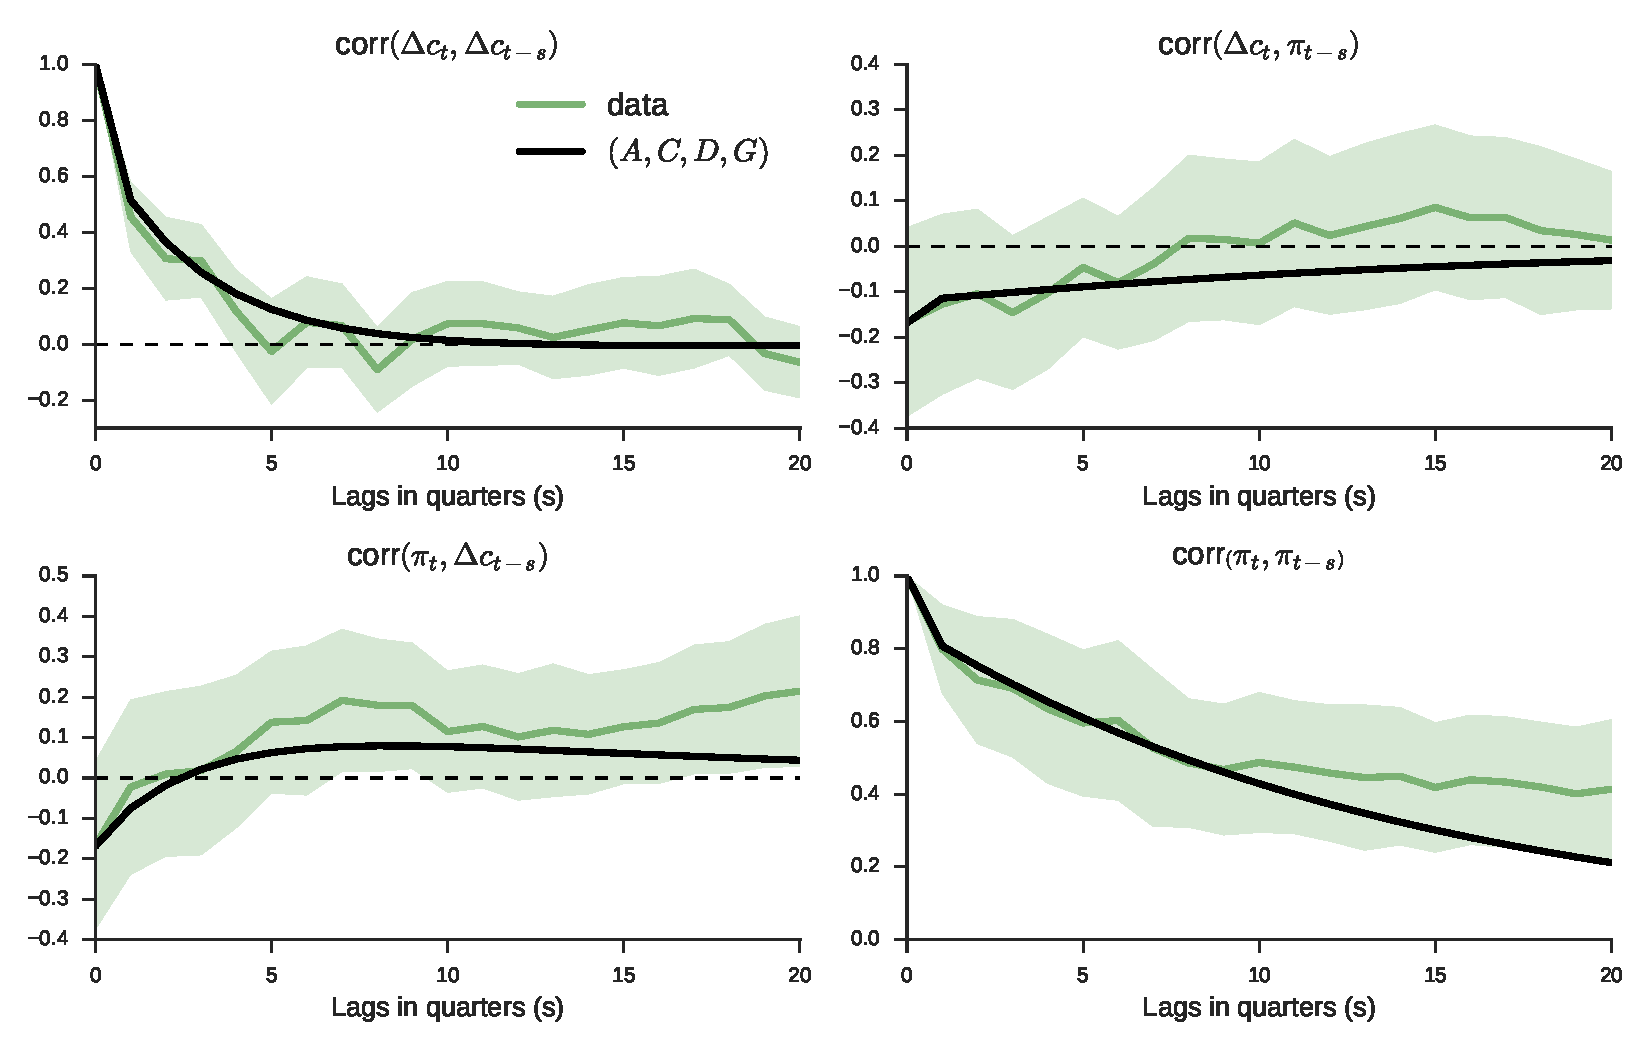
\includegraphics[width=\linewidth,keepaspectratio]{fig2_tom.pdf}
\caption{An econometrician's model of growth in aggregate consumption: estimated state dynamics.}
\label{fig:econometrician}
\end{figure}

\subsection{Risk-neutral rational expectations pricing}

Under rational expectations with a risk-neutral representative investor,
stock prices satisfy (Shiller):
\[
   p_t = \exp(-r_t)\, E_t\bigl( p_{t+1} + d_{t+1}\bigr).
\]
The expectations theory of the term structure of interest rates
(citet{Hicks1939}--Shiller) prices a zero-coupon risk-free claim to one dollar at
time $t+n$ as:
\begin{align}
p_t(1) &= \exp(-r_t), \notag\\
p_t(n+1) &= \exp(-r_t)\, E_t\, p_{t+1}(n), \label{eq:rn-recursion}\\
p_t(n) &= \exp(B_n\, x_t). \notag
\end{align}
These formulas work ``pretty well'' for conditional means but less well
for conditional variances---the Shiller ``volatility puzzles.''

\subsection{Modern asset pricing: adding risk aversion}
\label{sec:modern-ap}

It would be convenient if versions of the same formulas worked even when
investors are risk averse or do not have rational expectations.  The
likelihood ratio makes this possible.

Let
\begin{align}
m_{t+1}^\lambda &= \exp\!\left(-\lambda_t'\, \varepsilon_{t+1}
    - \tfrac{1}{2}\,\lambda_t'\lambda_t\right), \qquad
    \lambda_t = \lambda\, x_t, \label{eq:sdf-lr}\\
E_t\, m_{t+1}^\lambda &= 1, \qquad m_{t+1}^\lambda \geq 0. \notag
\end{align}
The likelihood ratio $m_{t+1}^\lambda$ distorts the conditional
distribution of $\varepsilon_{t+1}$ from ${\mathcal N}(0,I)$ to
${\mathcal N}(-\lambda\, x_t, I)$.  Covariances of returns with
$m_{t+1}^\lambda$ affect mean returns---this is the channel through
which risk aversion prices risks.

With this device, modern asset pricing (\citet{Lucas1978} for stocks,
\citet{DS2000}, \citet{cox1985theory}, and  \citet{BZ1994} for bonds) takes the form:
\begin{align}
p_t &= \exp(-r_t)\, E_t\bigl(
    {\color{red} m_{t+1}^\lambda}\,(p_{t+1} + d_{t+1})\bigr),
    \label{eq:stock-lr}
\end{align}
and for the term structure:
\begin{align}
p_t(1) &= \exp(-r_t), \notag\\
p_t(n+1) &= \exp(-r_t)\, E_t\bigl(
    {\color{red} m_{t+1}^\lambda}\, p_{t+1}(n)\bigr), \label{eq:ts-lr}\\
p_t(n) &= \exp(B_n\, x_t). \notag
\end{align}

\subsection{Risk-neutral dynamics}

The risk-neutral representation implies twisted dynamics:
\begin{align*}
x_{t+1} &= (A - {\color{red} C\lambda})\, x_t
    + C\, \tilde\varepsilon_{t+1}, \qquad
    \tilde\varepsilon_{t+1} \sim {\mathcal N}(0,I).
\end{align*}
The risk-neutral dynamics assert that the shock distribution
$\varepsilon_{t+1}$ has conditional mean $-\lambda_t$ instead of~$0$.
The dependence of $\lambda_t = \lambda\, x_t$ on the state modifies
the dynamics relative to the econometrician's model.

\subsection{Expectation under a twisted distribution}

The mathematical expectation of $y_{t+1}$ under the probability
distribution twisted by likelihood ratio $m_{t+1}$ is
\[
   \tilde E_t\, y_{t+1} = E_t\, m_{t+1}\, y_{t+1}.
\]
With respect to the risk-neutral dynamics, the term structure theory
becomes:
\begin{align*}
p_t(1) &= \exp(-r_t), \\
p_t(n+1) &= \exp(-r_t)\, \tilde E_t\, p_{t+1}(n), \\
p_t(n) &= \exp(\tilde B_n\, x_t).
\end{align*}
These are the same formulas as rational-expectations asset pricing, but
mathematical expectations are taken with respect to a probability
measure {\color{red} twisted by risk aversion}.


%% ====================================================================
\section{The Identification Challenge}
\label{sec:identification}
%% ====================================================================

The elegance of the likelihood ratio device comes at a cost: the same
mathematical object can represent very different economic forces.  This
section makes the observational equivalence precise.  Because asset
pricing formulas depend on~$\lambda_t$ but not on its interpretation,
the data alone cannot tell us whether observed risk premia reflect the
representative investor's risk aversion or systematically mistaken
beliefs.  Resolving this issue requires either additional data
or additional theory---the subjects of the sections that follow.

The vector $\lambda_t$ can be interpreted as either:
\begin{itemize}
\item a risk price vector expressing the representative agent's risk
      aversion, or
\item the representative agent's belief distortion relative to the
      econometrician's model.
\end{itemize}
The asset pricing formulas~\eqref{eq:stock-lr}--\eqref{eq:ts-lr} are
identical under both interpretations, and so are the econometric fits.
Relative to the model of a risk-averse representative investor with
rational expectations, a model of a risk-neutral investor with
appropriately mistaken beliefs produces observationally equivalent
predictions.  This insight was articulated by Hansen, Sargent, and
Tallarini~(1999) and Piazzesi, Salomao, and Schneider~(2015).

To distinguish risk aversion from belief distortion, one needs either
more information (the PSS approach using survey data) or more theory
(the Hansen and Sz\H{o}ke robust control approach), or both (Sz\H{o}ke).


%% ====================================================================
\section{More Information: Experts' Forecasts}
\label{sec:PSS}
%% ====================================================================

One natural strategy for breaking the identification deadlock is to
bring in additional data.  Piazzesi, Salomao, and Schneider~(2015)
pursue exactly this approach by exploiting surveys of professional
forecasters.  If forecasters' reported expectations differ
systematically from those implied by the econometrician's model, the
discrepancy can be attributed to belief distortions, leaving a smaller
residual to be explained by risk aversion alone.  This section describes
their framework and its empirical findings.

\subsection{The PSS framework}

Piazzesi, Salomao, and Schneider~(2015, henceforth PSS) exploit data on
professional forecasters' expectations to decompose the likelihood ratio
into risk prices and belief distortions.  Their setup posits:
\begin{itemize}
\item The representative agent's risk aversion leads him to price risks
      $\varepsilon_{t+1}$ with prices $\lambda_t^* = \lambda^*\, x_t$.
\item The representative agent has twisted beliefs
      $(A^*, C) = (A - C w^*, C)$ relative to the econometrician's model
      $(A, C)$.
\item Professional forecasters use the twisted beliefs $(A^*, C)$ to
      answer survey questions about their forecasts.
\end{itemize}

The question PSS assume experts think they are answering is: ``What
forecasts underlie your investment advice decisions?''

\subsection{Estimation strategy}

PSS proceed as follows:
\begin{enumerate}
\item Use data $\{x_t\}_{t=0}^T$ to estimate the econometrician's model
      $A$, $C$.
\item Project experts' forecasts $\{\hat x_{t+1}\}$ on $x_t$ to obtain
      $\hat x_{t+1} = A^*\, x_t$ and interpret $A^*$ as a belief
      distortion.
\item Back out the mean distortion
      $w^*\, x_t = -C^{-1}(A^* - A)\, x_t$ to the density of
      $\varepsilon_{t+1}$.
\item Reinterpret the $\lambda$ estimated by the rational-expectations
      econometrician as $\lambda = \lambda^* + w^*$, where
      $\lambda_t^* = \lambda^*\, x_t$ is the (smaller) price of risk
      vector actually charged by the representative agent with distorted
      beliefs.
\end{enumerate}

An econometrician who mistakenly imposes rational expectations estimates
risk prices $\lambda_t$ that sum two parts:
\begin{itemize}
\item smaller risk prices $\lambda_t^*$ actually charged by the
      erroneous-beliefs representative agent, and
\item conditional mean distortions $w_t^*$ of the risks
      $\varepsilon_{t+1}$ that the twisted-beliefs representative
      agent's model displays relative to the econometrician's.
\end{itemize}

\subsection{Empirical specification}

The key variables in PSS's state-space system are:
\begin{itemize}
\item the level and slope of the yield curve (short rate; spread between
      5-year and short rate),
\item inflation, and
\item conditional expectations of these variables.
\end{itemize}

\subsection{PSS successes}

PSS find $w^* \neq 0$:
\begin{itemize}
\item The experts' model differs systematically from the
      econometrician's.
\item Experts perceive the level and slope of the yield curve to be more
      persistent than the econometrician's estimates imply.
\item Subjective risk prices $\lambda^*\, x_t$ vary less than the
      $\lambda\, x_t$ estimated by the rational-expectations
      econometrician.
\end{itemize}

\subsection{Why are beliefs distorted?}

PSS offer no explanation for why beliefs are distorted.  Are they
mistakes?  Ignorance of good econometrics?  And how distorted are they
in terms of the divergence of probabilities?  These questions motivate a
theory of belief distortions rooted in robust control theory.

An intriguing interpretive question lurks here: are professional
forecasters reporting their best guess of the future, or the scenario
that rationalizes their portfolio decisions?  If the latter, their
``mistakes'' may not be mistakes at all but instead reflect a
pessimistic model that they use precisely because they fear
misspecification.  Section~\ref{sec:robust} develops a theory in which
this distinction is formalized: the robust control agent's worst-case
model generates forecasts that look like the experts' distorted beliefs,
but arise from an optimizing response to model uncertainty rather than
from ignorance.


%% ====================================================================
\section{Rational Expectations and Its Alternatives}
\label{sec:RE-limits}
%% ====================================================================

Before developing a theory of belief distortions, it is worth pausing to
ask why a rational expectations model might not be a good approximation.%
\footnote{Sargent~(2008) discusses the intellectual history of rational
expectations and adaptive learning, framing the tension between them as
one between ``intelligent design'' and ``evolution.''  The introduction
to Lucas and Sargent~(1981) lays out the case for rational expectations
as a discipline on econometric practice.}
The standard justification treats rational expectations as the outcome
of learning from a long history---but how long is long enough?  This
section reviews the conditions under which learning converges to
rational expectations and highlights circumstances, particularly those
involving persistent dynamics, in which convergence is so slow that
model uncertainty becomes economically first-order.

\subsection{The 1970s--1980s informal justification}

The standard justification for rational expectations treats it as the
outcome of learning from an infinite history: least-squares learning
converges to rational expectations.  The argument requires that:
\begin{itemize}
\item agents know correct functional forms, and
\item a stochastic approximation argument partitions dynamics into fast
      parts (justifying a law of large numbers) and slow parts
      (justifying an ODE).
\end{itemize}
However, long intertemporal dependencies make
{\color{red} rates of convergence slow}.
For example, distinguishing two Gaussian AR(1) processes whose
persistence parameters differ by $0.01$ (say $\rho = 0.98$ versus
$\rho = 0.99$) at the $5\%$ level requires several hundred years of
quarterly data.  For the long-run risk specifications considered by
Bansal and Yaron~(2004), the required sample lengths can exceed a
millennium.  This is not a failure of econometrics---it is the
statistical reality that makes model uncertainty economically important.

\subsection{Good econometricians}

Good econometricians have limited data and only hunches about functional
forms.  They fear that their fitted models are incorrect.  An agent who
is like a good econometrician:
\begin{itemize}
\item has a parametric model estimated from limited data,
\item acknowledges that many other specifications fit nearly as
      well---other parameter values, other functional forms, omitted
      variables, neglected nonlinearities, and history dependencies,
\item fears that one of those other models actually prevails, and
\item seeks ``good enough'' decisions under \emph{all} such alternative
      models---\emph{robustness}.
\end{itemize}


%% ====================================================================
\section{A Theory of Belief Distortions: Robust Control}
\label{sec:robust}
%% ====================================================================

Having seen that survey data point to systematic belief distortions and
that statistical theory explains why such distortions are hard to
eliminate through learning, we now develop a theory that rationalizes
them.  Robust control theory provides a framework in which a decision
maker who acknowledges that her model may be misspecified optimally
distorts her probability assessments toward a worst-case scenario.  The
resulting worst-case beliefs look like the ``mistakes'' identified by
PSS, but arise from a coherent response to model uncertainty rather than
from ignorance.

\subsection{Hansen's dubious agent}

Inspired by robust control theory, consider a dubious investor who:
\begin{itemize}
\item shares the econometrician's model $A$, $C$, $D$, $G$,
\item expresses doubts by using a continuum of likelihood ratios to form
      a \emph{discounted entropy ball} of size $\eta$ around the
      econometrician's model,
\item wants a valuation that is good for every model in the entropy
      ball, and
\item constructs a lower bound on values and a worst-case model that
      attains it.
\end{itemize}

\subsubsection{Why discounted entropy?}

Discounted entropy includes models that undiscounted entropy excludes.
Undiscounted entropy over infinite sequences excludes many models that
are very difficult to distinguish from the econometrician's model with
limited data, because undiscounted entropy includes only models that
share laws of large numbers.
To see why this matters, note that undiscounted entropy effectively
requires alternative models to share the same long-run averages as the
baseline---it excludes models that differ only in persistent,
low-frequency dynamics.
But those are precisely the models that are hardest to distinguish with
finite data and that matter most for long-lived asset prices.
Discounted entropy, by treating future divergences less severely, admits
these statistically elusive but economically important alternatives into
the set of models that the dubious agent contemplates.

\subsection{Valuation under the econometrician's model}

Taking the log consumption process to be linear Gaussian with shocks
$\varepsilon_{t+1} \sim {\mathcal N}(0,I)$:
\begin{align}
c_{t+1} - c_t &= D\, x_t + G\, \varepsilon_{t+1}, \label{eq:cons}\\
x_{t+1} &= A\, x_t + C\, \varepsilon_{t+1}, \label{eq:state2}
\end{align}
the value function is
\[
   V(x_0, c_0) := E\!\left[\sum_{t=0}^{\infty} \beta^t\, c_t
       \;\middle|\; x_0, c_0\right]
   = c_0 + \beta\, E\!\left[V(x_1, c_1)
       \;\middle|\; x_0, c_0\right].
\]

\subsection{The sequence problem}

The dubious agent solves:
\begin{align}
J(x_0, c_0 \mid \eta) &:= \min_{\{m_{t+1}\}_{t=0}^\infty}
    E\!\left[\sum_{t=0}^{\infty} \beta^t\,
    {\color{orange} M_t}\, c_t \;\middle|\; x_0, c_0\right]
    \label{eq:hansen-seq}\\
&\quad \text{s.t.}\quad
    c_{t+1} - c_t = D\, x_t + G\, \varepsilon_{t+1}, \notag\\
&\quad\hphantom{\text{s.t.}}\quad
    x_{t+1} = A\, x_t + C\, \varepsilon_{t+1}, \notag\\
&\quad\hphantom{\text{s.t.}}\quad
    E\!\left[\sum_{t=0}^{\infty} \beta^t\, M_t\,
    E\!\left[m_{t+1}\log m_{t+1} \;\middle|\; x_t, c_t\right]
    \;\middle|\; x_0, c_0\right] \leq {\color{orange} \eta}, \notag\\
&\quad\hphantom{\text{s.t.}}\quad
    M_{t+1} = M_t\, m_{t+1},\quad
    E[m_{t+1} \mid x_t, c_t] = 1,\quad M_0 = 1. \notag
\end{align}
The likelihood ratio process $\{M_t\}_{t=0}^\infty$ is a multiplicative
{\color{red} martingale}.

\begin{figure}[t]
\centering
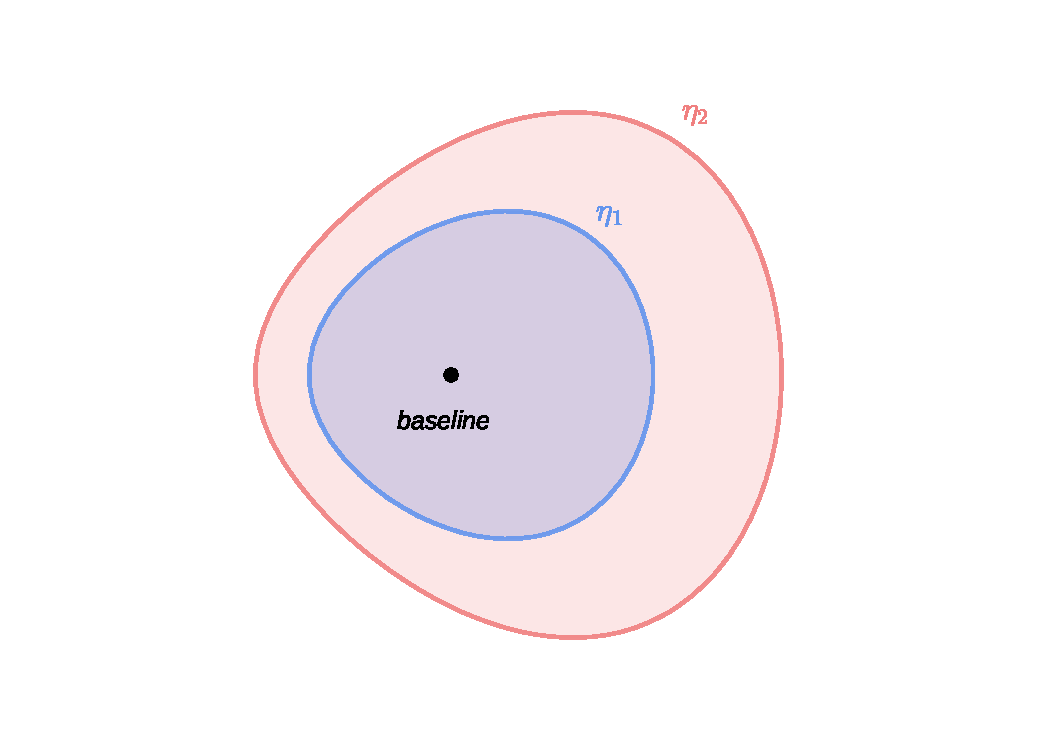
\includegraphics[width=0.85\textwidth]{eggs_backus.pdf}
\caption{Discounted entropy ball around the econometrician's model.}
\label{fig:entropy-ball}
\end{figure}

\subsection{Entropy and the likelihood ratio}

With the log-normal likelihood ratio
\[
   m_{t+1} := \exp\!\left(- w_t'\, \varepsilon_{t+1}
       - \tfrac{w_t' w_t}{2}\right),
\]
conditional entropy takes the simple form
\[
   E\!\left[m_{t+1}\log m_{t+1} \;\middle|\; x_t, c_t\right]
       = \tfrac{1}{2}\, w_t' w_t.
\]
Substituting this into~\eqref{eq:hansen-seq} yields the reformulated
problem:
\begin{align}
J(x_0, c_0 \mid \eta) &:= \min_{\{w_t\}_{t\geq 0}}
    E^w\!\left[\sum_{t=0}^{\infty} \beta^t\, c_t
    \;\middle|\; x_0, c_0\right] \label{eq:hansen-seq2}\\
&\quad \text{s.t.}\quad
    c_{t+1} - c_t = D\, x_t + G\,(\tilde\varepsilon_{t+1}
    - {\color{orange} w_t}), \qquad
    \tilde\varepsilon_{t+1} \sim {\mathcal N}(0,I), \notag\\
&\quad\hphantom{\text{s.t.}}\quad
    x_{t+1} = A\, x_t + C\,(\tilde\varepsilon_{t+1}
    - {\color{orange} w_t}), \notag\\
&\quad\hphantom{\text{s.t.}}\quad
    \tfrac{1}{2}\, E^w\!\left[\sum_{t=0}^{\infty} \beta^t\,
    w_t' w_t \;\middle|\; x_0, c_0\right] \leq
    {\color{orange} \eta}. \notag
\end{align}

\subsection{Outcome of the Hansen model}

The worst-case mean distortion turns out to be a constant vector:
\[
   w_t = \bar w.
\]
The consequence is that the contribution of $w_t$ to risk prices is
state-independent.  This does \emph{not} help explain countercyclical
prices of risk (or prices of model uncertainty).


%% ====================================================================
\section{Tilting the Entropy Ball}
\label{sec:tilted}
%% ====================================================================

The basic robust control model of the previous section has a limitation:
it generates worst-case distortions that are constant across states, and
therefore cannot explain the countercyclical variation in risk prices
that the data demand.  This section shows how Hansen and Sz\H{o}ke
overcome this limitation by \emph{tilting} the entropy ball---requiring
it to include particular parametric alternatives, such as models with
more long-run risk.  The tilt makes the entropy constraint bind
differently across states, producing the state-dependent uncertainty
prices needed to match term-structure dynamics.

\subsection{Hansen and Sz\H{o}ke's more refined dubious agent}

To generate state-dependent uncertainty prices, Hansen and Sz\H{o}ke
introduce a more refined dubious agent who:
\begin{itemize}
\item shares the econometrician's model $A$, $C$, $D$, $G$,
\item expresses doubts by using a continuum of likelihood ratios to form
      a discounted entropy ball around the econometrician's model,
\item also insists that some martingales representing particular
      alternative \emph{parametric} models be included in the
      discounted entropy ball.
\end{itemize}
The inclusion of those alternative parametric models \emph{tilts} the
entropy ball, which affects the worst-case model in a way that can
produce countercyclical uncertainty prices.

\subsection{Concern about other parametric models}

The investor wants to include particular alternative models with
\[
   E_t\!\left[\bar m_{t+1}\log\bar m_{t+1}\right]
       = \tfrac{1}{2}\,\bar w_t'\,\bar w_t = \xi(x_t)
\]
and discounted entropy
\[
   E^{\bar w}\!\left[\sum_{t=0}^{\infty} \beta^t\,\xi(x_t)
       \;\middle|\; x_0, c_0\right].
\]
This is accomplished by replacing the earlier entropy constraint with
\begin{equation}
\tfrac{1}{2}\, E^w\!\left[\sum_{t=0}^{\infty} \beta^t\, w_t' w_t
    \;\middle|\; x_0, c_0\right]
    \leq E^w\!\left[\sum_{t=0}^{\infty} \beta^t\,\xi(x_t)
    \;\middle|\; x_0, c_0\right].
\label{eq:tilted-constraint}
\end{equation}

\subsection{Bansal and Yaron's bazooka}

Bansal and Yaron~(2004) mix long-run risk (LRR) with Epstein--Zin (EZ)
preferences.\footnote{Dave Backus dubbed Bansal and Yaron's idea of combining two hypotheses -- the
presence of long run risk in consumption growth together with a representative agent who hates long-run risk --
as a `bazooka' because of the powerful way it raised market prices of risk.}   LRR is statistically difficult to detect and estimate, but
an Epstein--Zin agent or a dubious agent really hates LRR.  Under
certain conditions, the EZ value function is the indirect utility
function of a dubious agent.  This sets the stage for big risk
prices---but not countercyclical ones.

\begin{remark}[EZ--robust control equivalence]
The equivalence between Epstein--Zin preferences and robust control,
established by Hansen and Sargent~(2001) and Maenhout~(2004), implies
that EZ preferences with unit elasticity of intertemporal substitution
and risk aversion $\gamma > 1$ are observationally equivalent to expected
utility with $\gamma = 1$ combined with a penalty parameter
$\theta = 1/(\gamma - 1)$ governing robustness.  The higher the risk
aversion under EZ, the smaller the entropy ball the robust agent is
willing to tolerate---she fears a narrower but more intense set of model
misspecifications.
\end{remark}

\subsection{Concern about bigger long-run risk in the Sz\H{o}ke model}

Inspired by Bansal and Yaron~(2004), an agent fears particular long-run
risks expressed by
\[
   x_{t+1} = \bar A\, x_t + C\,\tilde\varepsilon_{t+1}.
\]
This corresponds to $\bar w_t = \bar w\, x_t$ with
\[
   \bar w = -C^{-1}(\bar A - A),
\]
which implies a quadratic $\xi$ function:
%\[
%   \xi(x_t) := x_t'\,\bar w'\,\bar w\, x_t =: x_t'\,\Xi\, x_t.
%\]
\[
   \xi(x_t) := \frac{1}{2} x_t'\,\bar w'\,\bar w\, x_t =: \frac{1}{2} x_t'\,\Xi\, x_t.
\]

\begin{figure}[t]
\centering
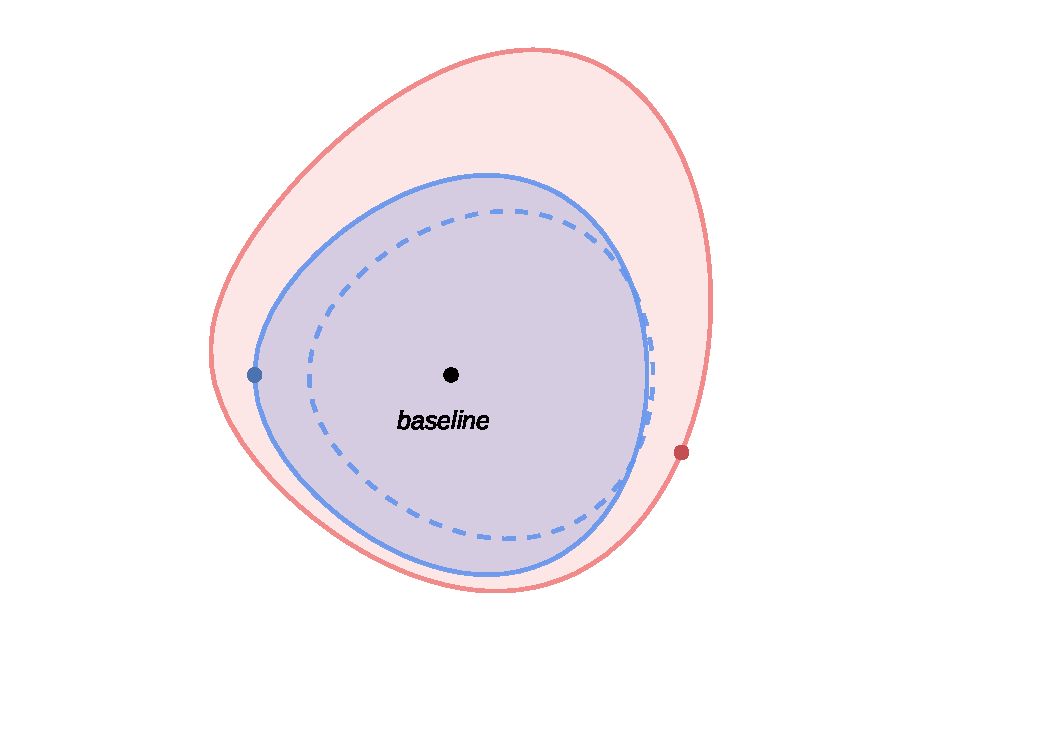
\includegraphics[width=0.85\textwidth]{eggs_backus2.pdf}
\caption{Tilted discounted entropy balls.  Including particular
parametric alternatives with more long-run risk tilts the entropy ball
and generates state-dependent worst-case distortions.}
\label{fig:tilted-entropy}
\end{figure}

\subsection{State-dependent contributions to the entropy constraint}

The time-$t$ contributions to the right-hand side
of~\eqref{eq:tilted-constraint} relax the discounted entropy constraint
in states $x_t$ in which $\xi(x_t)$ is larger.  This sets the stage for
state-dependent mean distortions in the worst-case model, which in turn
ignite countercyclical market prices of uncertainty.

\subsection{The Sz\H{o}ke agent's sequence problem}

The resulting linear-quadratic problem is:
\begin{align}
J(x_0, c_0 \mid \Xi) &:= \max_{\tilde\theta \geq 0}\;
    \min_{\{w_t\}_{t\geq 0}}\;
    E^w\!\left[\sum_{t=0}^{\infty} \beta^t\, c_t
    + \tilde\theta\, \tfrac{1}{2}\sum_{t=0}^{\infty} \beta^t
    \bigl(w_t' w_t - x_t'\,\Xi\, x_t\bigr)
    \;\middle|\; x_0, c_0\right] \label{eq:szoke-seq}\\
&\quad \text{s.t.}\quad
    c_{t+1} - c_t = D\, x_t + G\,(\tilde\varepsilon_{t+1}
    - {\color{orange} w_t}), \qquad
    \tilde\varepsilon_{t+1} \sim {\mathcal N}(0,I), \notag\\
&\quad\hphantom{\text{s.t.}}\quad
    x_{t+1} = A\, x_t + C\,(\tilde\varepsilon_{t+1}
    - {\color{orange} w_t}). \notag
\end{align}
The worst-case shock mean distortion
 is\footnote{We have assumed that first entry in the the state vector is a constant $1$ so that 
 $x_t = \begin{bmatrix} 1 \cr \check x_t \end{bmatrix}$ where 
 $A = \begin{bmatrix} 1 & 0 \cr 0 & \check A \end{bmatrix} $ and $\check A$ is a stable matrix.
 Consequently, the worst-case distortion is now affine the stochastic part $\check x_t$ of the state vector:
$$
\tilde{w}_t = a + \check {W} \check x_t
$$
where $a$ is a constant vector determined by the linear terms in the value function.
When $\Xi = 0$ (no tilting), the constant $a$ reduces to the Hansen $\bar{w}$ from the untilted problem.
However, when $\Xi \neq 0$ the two differ because the quadratic value function contributes an additional $2\beta C^\top \Xi C$ term to the left-hand side of the first-order condition for the constant part. The state-dependent component $\check{W} \check x_t$ is the new contribution of the tilted entropy ball, and is what generates countercyclical uncertainty prices. }
\[
   \tilde w_t = \widetilde W\, x_t,
\]
and the worst-case model is $(\tilde A, C, \tilde D, G)$ with
\begin{align*}
\tilde A &= A - C\,\tilde W, \\
\tilde D &= D - G\,\tilde W.
\end{align*}


%% ====================================================================
\section{Empirical Results}
\label{sec:empirics}
%% ====================================================================

We now confront the theoretical framework with data.  This section
reviews the key empirical patterns in the U.S.\ term structure of
interest rates---the upward-sloping yield curve, the predictive power of
the yield spread for recessions, and Shiller's volatility puzzle---and
assesses how well different models account for them.  The centerpiece is
Sz\H{o}ke's~(2022) estimation of the tilted entropy ball model, which
imposes cross-equation restrictions linking the worst-case model to both
bond prices and survey forecasts.

\subsection{The U.S.\ term structure}

\begin{figure}[t]
\centering
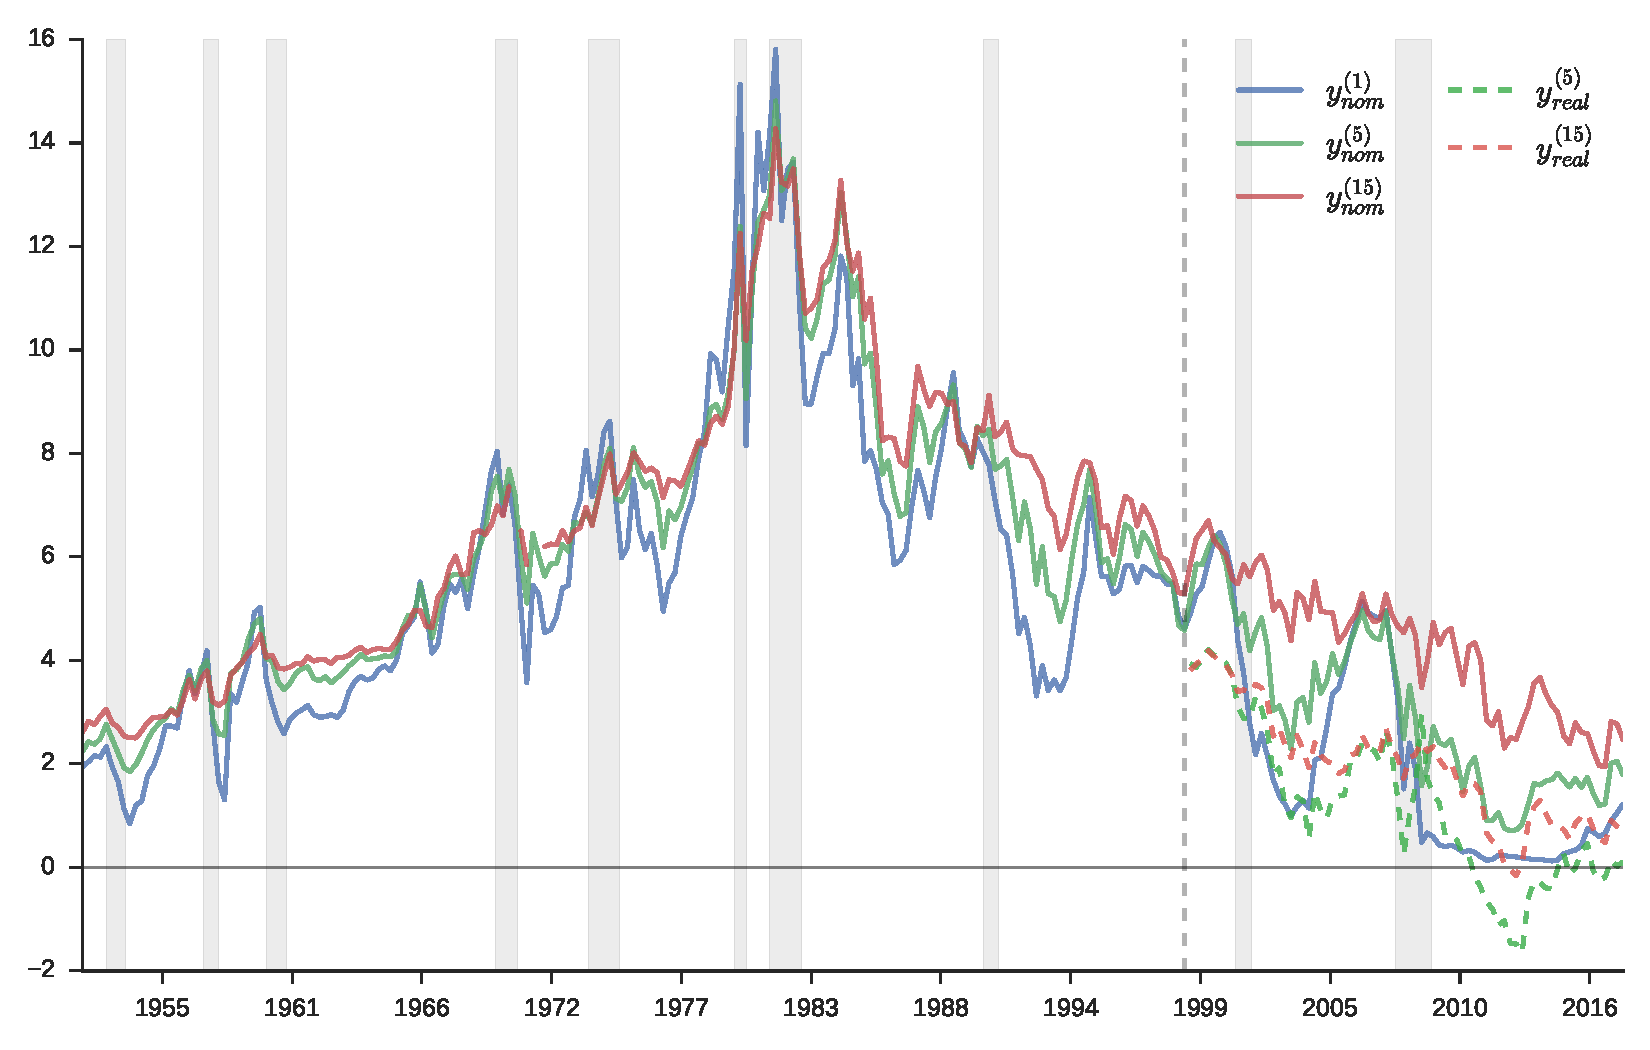
\includegraphics[width=\linewidth,keepaspectratio]{fig1_tom.pdf}
\caption{U.S.\ term structure of interest rates.}
\label{fig:us-term}
\end{figure}

Several recognized patterns characterize the U.S.\ term structure:
\begin{itemize}
\item The nominal yield curve usually slopes upward.
\item The long-minus-short yield spread narrows before U.S.\ recessions
      and widens after them.
\item Consequently, the slope of the yield curve helps predict aggregate
      inputs and outputs.
\item Long and short yields are almost equally volatile (the ``Shiller
      puzzle'').
\item To solve the Shiller puzzle, risk prices (or something
      observationally equivalent) must depend on volatile state
      variables.
\end{itemize}

Specific historical episodes bring these patterns to life.  The yield
curve inverted before each of the last seven U.S.\ recessions.
In the Sz\H{o}ke model, inversions correspond to states where
$\xi(x_t)$ is small---the agent's long-run risk worry is muted---which
tightens the entropy constraint and compresses risk prices.
Conversely, during the 2008--09 financial crisis and the March~2020
COVID shock, term premia spiked as uncertainty about long-run
consumption growth surged, exactly the pattern that the tilted entropy
ball is designed to capture.

\subsection{Challenges and responses}

Table~\ref{tab:challenges} summarizes how various models perform against
these empirical challenges.

\begin{table}[H]
\begin{center}
\begin{tabular}{lccc}
& Average   & Slopes near  & Volatile\\
& slope    & recessions & long yield \\
\hline\\[-6pt]
Lucas (1978)  &  no & no & no \\[4pt]
Epstein--Zin with LRR & maybe & yes & no \\
\quad (PS (2007), HS (2001)) & & & \\[4pt]
PSS (2015) &  built-in  &  built-in & yes \\[4pt]
Sz\H{o}ke (2022) & YES  & yes & yes \\[4pt]
\end{tabular}
\end{center}
\caption{Challenges and model performances.  Affine risk prices with
persistent consumption growth can address the second column; the third
column requires state-dependent prices of risk.}
\label{tab:challenges}
\end{table}

\subsection{Sz\H{o}ke's empirical strategy}

Sz\H{o}ke proceeds in two stages:

\paragraph{Stage~I: Estimation.}
\begin{enumerate}
\item Use $\{x_t, c_t\}_{t=0}^T$ to estimate the econometrician's
      $A$, $C$, $D$, $G$.
\item View $\Xi$ as a matrix of additional free parameters and estimate
      them simultaneously with risk prices $\tilde\lambda\, x_t$ from
      data $\{p_t(n+1)\}_{n=1}^N$, $t = 0, \ldots, T$, by imposing
      cross-equation restrictions:
%\begin{align}
%p_t(n+1) &= \exp(-r_t)\, E_t\!\left[
%    m_{t+1}^{\tilde w}\, m_{t+1}^{\tilde\lambda}\,
%    p_{t+1}(n)\right], \label{eq:szoke-pricing}\\
%m_{t+1}^{\tilde w} &= \exp\!\left(-\tilde w_t'\,\varepsilon_{t+1}
%    - \tfrac{\tilde w_t'\,\tilde w_t}{2}\right), \notag\\
%m_{t+1}^{\tilde\lambda} &= \exp\!\left(-\tilde\lambda_t'\,
%    \varepsilon_{t+1}
%    - \tfrac{\tilde\lambda_t'\,\tilde\lambda_t}{2}\right), \notag
%\end{align}
\begin{align}
p_t(n+1) &= \exp(-r_t)\, E_t\!\left[
    m_{t+1}^{\rm total} \, %m_{t+1}^{\tilde w}\, m_{t+1}^{\tilde\lambda}\,
    p_{t+1}(n)\right], \label{eq:szoke-pricing}\\
m_{t+1}^{\rm total} &= \exp\left( - (\tilde w_t +\tilde \lambda_t)' \varepsilon_{t+1} - \frac{1}{2} || \tilde w_t +\tilde \lambda_t||^2 \right)
\notag
%
%\exp\!\left(-\tilde w_t'\,\varepsilon_{t+1}
%    - \tfrac{\tilde w_t'\,\tilde w_t}{2}\right), \notag\\
%m_{t+1}^{\tilde\lambda} &= \exp\!\left(-\tilde\lambda_t'\,
%    \varepsilon_{t+1}
%    - \tfrac{\tilde\lambda_t'\,\tilde\lambda_t}{2}\right), \notag
\end{align}
where $E_t$ is taken with respect to the econometrician's model and
$\tilde w_t = \tilde W\, x_t$ is the dubious investor's worst-case
model.
\end{enumerate}

\paragraph{Stage~II: Assessment.}
\begin{enumerate}
\item Assess improvements in predicted behavior of the term structure.
\item Use estimated worst-case dynamics to form distorted forecasts
      $\tilde x_{t+1} = (A - C\,\tilde W)\, x_t$ and compare them to
      those of professional forecasters.
\item Compute discounted relative entropy of the worst-case twisted
      model $(A - C\,\tilde W, C, D - G\,\tilde W, G)$ relative to the
      econometrician's model $(A,C,D,G)$, and use it together with
      Chernoff--Newman--Stuck entropy measures to assess the difficulty
      of distinguishing the two models.
\end{enumerate}

\subsection{Interpretations of conditional mean distortions}

The conditional mean distortions $w\, x_t$ admit distinct
interpretations:
\begin{itemize}
\item In PSS, $w_t^*$ is a vector of ``mistakes'' or ``suboptimal
      forecasts.''
\item In Sz\H{o}ke, $\tilde w_t$ is a vector of ``model uncertainty''
      prices: compensations the representative agent charges to bear
      risks $\varepsilon_{t+1}$ with unknown probability distribution.
\end{itemize}

\subsection{Insights from Sz\H{o}ke's model}

Sz\H{o}ke's framework delivers:
\begin{enumerate}
\item A theory of state-dependent belief distortions
      $\tilde w_t = \tilde W\, x_t$.
\item A theory about the question that professional forecasters answer:
      they respond with their worst-case model because they hear ``tell
      me forecasts that rationalize your (max-min) decisions.''
\item A way to measure the size of belief distortions relative to the
      econometrician's model.
\end{enumerate}

He uses his estimated $\Xi$ matrix:
\begin{itemize}
\item to infer an equivalence class of alternative parametric models
      parameterized by $\bar w$ that concern the representative
      investor---these models have more long-run risk than the
      econometrician's model;
\item to infer a worst-case mean distortion $\tilde W\, x_t$ whose
      state dependence causes the term structure to move with $x_t$ in
      ways that explain hitherto puzzling term-structure movements,
      including Shiller's ``volatility puzzle.''
\end{itemize}

\subsection{Three probability twisters}

To summarize, three distinct probability twisters play roles in this
analysis:
\begin{itemize}
\item $w_t^*$: Piazzesi, Salomao, and Schneider's mistaken agent;
\item $\bar w_t$: Sz\H{o}ke's especial LRR parametric concern;
\item $\tilde w_t$: Sz\H{o}ke's worst-case model.
\end{itemize}


%% ====================================================================
\section{Cross-Equation Restrictions and Estimation}
\label{sec:motivation}
%% ====================================================================

A recurring theme throughout the rational expectations econometrics
literature is that equilibrium models impose testable restrictions across
the equations of a vector autoregression.\footnote{See Lucas and Sargent~(1981).}  
This section highlights how
the robust control framework preserves that desirable feature: even
though the decision maker's beliefs depart from the econometrician's
model, the departure is disciplined by the worst-case optimization
problem, yielding a new but equally sharp set of cross-equation
restrictions that can be taken to the data.

A key appeal of the robust control approach is that it lets us deviate
from rational expectations while still preserving a set of powerful
cross-equation restrictions on decision makers' beliefs.
Hansen and Sargent~(1991) provided systematic methods for deriving and
imposing the cross-equation restrictions on vector autoregressions that
are implied by exact linear rational expectations models; those methods
set the stage for the estimation strategy used here.
As Sz\H{o}ke puts it:
\begin{quote}
An appealing feature of robust control theory is that it lets us deviate
from rational expectations, but still preserves a set of powerful
cross-equation restrictions on decision makers' beliefs\ldots\
Consequently, estimation can proceed essentially as with rational
expectations econometrics.  The main difference is that now restrictions
through which we interpret the data emanate from the decision maker's
best response to a worst-case model instead of to the econometrician's
model.
\end{quote}


%% ====================================================================
\section{Who Cares?}
\label{sec:conclusion}
%% ====================================================================

Joint probability distributions of interest rates and macroeconomic
shocks are important throughout macroeconomics:
\begin{itemize}
\item \textbf{Costs of aggregate fluctuations.}  Welfare assessments of
      business cycles depend sensitively on how risks are priced.
      Lucas~(1987) calculated the welfare cost of business cycles at
      roughly $0.05\%$ of lifetime consumption under standard risk
      aversion.  But if the representative agent fears model
      misspecification in the sense formalized above, that cost can rise
      by one or two orders of magnitude (Hansen, Sargent, and
      Tallarini~1999), because the agent evaluates fluctuations under a
      pessimistic probability model that amplifies downside risk.
\item \textbf{Consumption Euler equations.}  The ``New Keynesian IS
      curve'' is a log-linearized consumption Euler equation whose risk
      adjustments are controlled by the stochastic discount factor.
\item \textbf{Optimal taxation and government debt management.}
       Government bond prices embed risk prices whose state dependence
       matters for optimal fiscal policy.
\item \textbf{Central bank expectations management.}  Forward guidance
      works by shifting the term structure, an exercise whose effects
      depend on the same likelihood ratios studied here.
\item \textbf{Long-run risk and secular stagnation.}  The Bansal--Yaron
      long-run risk hypothesis is difficult to detect statistically, yet
      an agent who fears it in the sense formalized above may behave
      very differently than one who does not.
\end{itemize}

Understanding whether observed asset prices reflect risk aversion,
mistaken beliefs, or fears of model misspecification---and quantifying
each component---matters for both positive and normative
macroeconomics.


%% ====================================================================
%% Appendix
%% ====================================================================
\appendix
\section{Multiplier Preferences}
\label{sec:multiplier}

The multiplier preference version of the dubious agent's problem is:
\begin{align}
W(x_0, c_0 \mid \theta) &:= \min_{\{m_{t+1}\}_{t\geq 0}}
    E\!\left[\sum_{t=0}^{\infty} \beta^t\,
    {\color{orange} M_t}\bigl(c_t + \theta\, m_{t+1}\log m_{t+1}\bigr)
    \;\middle|\; x_0, c_0\right], \label{eq:mult-seq}\\
&\quad M_{t+1} = M_t\, m_{t+1},\quad
    E[m_{t+1} \mid x_t, c_t] = 1,\quad M_0 = 1. \notag
\end{align}
The recursive formulation is:
\begin{align}
W(x_t, c_t \mid \theta) &= c_t + \min_{m_{t+1}}\;
    E\!\left[m_{t+1}\bigl[\beta W(x_{t+1}, c_{t+1})
    + \theta\log m_{t+1}\bigr] \;\middle|\; x_t, c_t\right] \notag\\
&= c_t - \theta\log E\!\left[\exp\!\left(
    -\frac{\beta W(x_{t+1}, c_{t+1})}{\theta}\right)
    \;\middle|\; x_t, c_t\right] \notag\\
&=: c_t + T_t\!\left[\beta W(x_{t+1}, c_{t+1})\right], \label{eq:mult-bellman}
\end{align}
where the right-hand side is attained by
\[
   m_{t+1}^* \propto \exp\!\left(
       -\frac{\beta W(x_{t+1}, c_{t+1})}{\theta}\right).
\]

\paragraph{Relationship between multiplier and constraint problems.}
By Lagrange multiplier theory,
\[
   W(x_t, c_t \mid \tilde\theta) = J(x_t, c_t \mid \eta)
       + \tilde\theta\, \eta.
\]


%% ====================================================================
%% References
%% ====================================================================
\begin{thebibliography}{99}

\bibitem[Backus et~al.(2001)]{BFT2001}
Backus, D.\,K., S.\ Foresi, and C.\,I.\ Telmer (2001).
``Affine term structure models and the forward premium anomaly,''
\textit{Journal of Finance} 56, 279--304.

\bibitem[Backus and Zin(1994)]{BZ1994}
Backus, D.\,K.\ and S.\,E.\ Zin (1994).
``Reverse engineering the yield curve,''
NBER Working Paper No.\ 4676.

\bibitem[Bierwag and Grove(1967)]{bierwag1967model}
Bierwag, Gerald O. and M.A. Grove (1967). "A model of the term structure of interest rates." \textit{The Review of Economics and Statistics}, 49(1), 50--62.

\bibitem[Bansal and Yaron(2004)]{BY2004}
Bansal, R.\ and A.\ Yaron (2004).
``Risks for the long run: A potential resolution of asset pricing puzzles,''
\textit{Journal of Finance} 59, 1481--1509.

\bibitem[Cox et~al.(1985)]{cox1985theory}
Cox, J.\,C., J.\,E.\ Ingersoll, and S.\,A.\ Ross (1985).
``A theory of the term structure of interest rates,''
\textit{Econometrica} 53, 385--407.

\bibitem[Dai and Singleton(2000)]{DS2000}
Dai, Q.\ and K.\,J.\ Singleton (2000).
``Specification analysis of affine term structure models,''
\textit{Journal of Finance} 55, 1943--1978.

\bibitem[Hansen and Sargent(1991)]{HansenSargent1991}
Hansen, L.\,P.\ and T.\,J.\ Sargent (1991).
``Exact linear rational expectations models: Specification and
estimation,''
in L.\,P.\ Hansen and T.\,J.\ Sargent (eds.),
\textit{Rational Expectations Econometrics},
Boulder, CO: Westview Press.
%
%\bibitem[Hansen and Sargent(2019)]{hansen2019exact}
%Hansen, L.\,P.\ and T.\,J.\ Sargent (2019).
%``Exact linear rational expectations models: Specification and
%estimation,'' in \textit{Rational Expectations Econometrics},
%pp.\ 45--75. CRC Press.

\bibitem[Hansen and Sargent(2001)]{HS2001}
Hansen, L.\,P.\ and T.\,J.\ Sargent (2001).
``Robust control and model uncertainty,''
\textit{American Economic Review} 91, 60--66.

\bibitem[Hansen et~al.(2020)]{HSHS2020}
Hansen, L.\,P., B.\ Sz\H{o}ke, L.\,S.\ Han, and T.\,J.\ Sargent (2020).
``Twisted probabilities, uncertainty, and prices,''
\textit{Journal of Econometrics} 216, 151--174.

\bibitem[Hansen et~al.(1999)]{HST1999}
Hansen, L.\,P., T.\,J.\ Sargent, and T.\,D.\ Tallarini (1999).
``Robust permanent income and pricing,''
\textit{Review of Economic Studies} 66, 873--907.

\bibitem[Hicks(1939)]{Hicks1939}
Hicks, J.\,R.\ (1939).
\textit{Value and Capital}.
Oxford: Clarendon Press.

\bibitem[Lucas(1978)]{Lucas1978}
Lucas, R.\,E.\ (1978).
``Asset prices in an exchange economy,''
\textit{Econometrica} 46, 1429--1445.

\bibitem[Lucas(1987)]{Lucas1987}
Lucas, R.\,E.\ (1987).
\textit{Models of Business Cycles}.
Oxford: Basil Blackwell.

\bibitem[Lucas and Sargent(1981)]{LucasSargent1981}
Lucas, R.\,E.\ and T.\,J.\ Sargent (eds.) (1981).
\textit{Rational Expectations and Econometric Practice}.
Minneapolis: University of Minnesota Press.

\bibitem[Maenhout(2004)]{Maenhout2004}
Maenhout, P.\,J.\ (2004).
``Robust portfolio rules and asset pricing,''
\textit{Review of Financial Studies} 17, 951--983.


\bibitem[Meiselman(1961)]{meiselman1961term}
Meiselman, David I. (1961). "The term structure of interest rates." Ph.D. thesis, University of Chicago.


\bibitem[Piazzesi and Schneider(2007)]{PS2007}
Piazzesi, M.\ and M.\ Schneider (2007).
``Equilibrium yield curves,''
\textit{NBER Macroeconomics Annual} 21, 389--442.

\bibitem[Piazzesi et~al.(2015)]{PSS2015}
Piazzesi, M., J.\ Salomao, and M.\ Schneider (2015).
``Trend and cycle in bond premia,''
Working Paper, Stanford University.

\bibitem[Sargent(2008)]{Sargent2008}
Sargent, T.\,J.\ (2008).
``Evolution and intelligent design,''
\textit{American Economic Review} 98, 5--37.

\bibitem[Sargent(1972)]{Sargent1972}
Sargent, T.\,J.\ (1972).
``Rational expectations and the term structure of interest rates,''
\textit{Journal of Money, Credit and Banking} 4, 74--97.

\bibitem[Sargent(1979)]{Sargent1979}
Sargent, T.\,J.\ (1979).
``A note on maximum likelihood estimation of the rational expectations
model of the term structure,''
\textit{Journal of Monetary Economics} 5, 133--143.

\bibitem[Shiller(1979)]{Shiller1979}
Shiller, R.\,J.\ (1979).
``The volatility of long-term interest rates and expectations models of
the term structure,''
\textit{Journal of Political Economy} 87, 1190--1219.

\bibitem[Sz\H{o}ke(2022)]{Szoke2022}
Sz\H{o}ke, B.\ (2022).
``Estimating robustness,''
\textit{Journal of Economic Theory} 199, 105225.

\end{thebibliography}


\end{document}
